\chapter{Marketing}

\epigraph{Dalla mattina alla sera,\\ da Stradella a Voghera.}{Slogan}
\section{An introduction to marketing strategies}
Setting up an effective marketing campaign is of paramount importance for a Company operating in any sector to launch a new product or service. The mobility sector is not an exception, a new transport service, even if properly scheduled, efficient under the O\&M point-of-view, and profitable on paper, remains under-utilized if potential customers don’t know about its existence.

The available budget for this kind of activities is often quite modest; therefore, the risk is to spend the resources in not an effective way, targeting the wrong customers or the wrong area.

The goal of this section is to present how the Team has decided to spend the $10000$ € budget made available by the company, explaining in detail the choices that guided the decisions, the selected marketing tools to make the people informed about the new service and finally what are the main KPI’s and how the Company could monitor the status of the campaign.

\paragraph{Target and area of interest}
Before starting with the actual marketing strategy, it is worth to carefully identify the border of the area that will be touched, along with the targets of the campaign.

The almost totality of the budget will be dedicated to the area of Pavia Province, mainly to the municipality of Voghera and to the Business Park area, where the launch event of the new service will take place (see next chapter).

Regarding the target, the strategy has as a goal to inform ideally each of the current employees and workers of the Park about the introduction of the new transport service. Being a service essentially dedicated to them, it has been considered convenient to reserve the largest part of the resources to the people that are spending their time inside the Business Park.

Therefore, a successful marketing campaign will be the one that persuades the largest number of employees to abandon their current mean of transport, to reach their workplace with the service offered by Autoguidovie. 

\paragraph{Market Strategy}
The selected strategy is a mix of “online” and “offline” tools revolving around a core event that will provide the participants the chance to touch with their hands the operability of the new service. The following scheme presents the structure of the entire strategy adopted.

\begin{figure}[h]
    \centering
    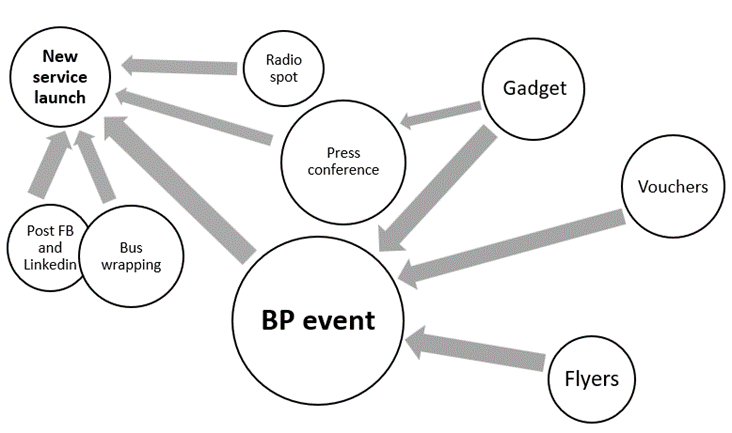
\includegraphics[width=0.7\textwidth]{Images/merketing/Strategy.png}
    \caption{Marketing Strategy}
    \label{fig:strategy}
\end{figure}

Each of the mentioned strategy, will be carefully described in a subsequent paragraph.

\section{KPI's and Costs of the strategies}
The initiatives abovementioned have obviously a cost for the Company, both in terms of financial resources and time to organize them. For this reason, it is fundamental to be able to monitor the effectiveness of these strategies through a proper set of KPI’s, to eventually adjust any decision that has previously been taken, and also to generate a record which could be useful for future marketing campaigns.

In the Table \ref{tab:marketing_strategy}, the reader can take a global look at the strategies, along with the KPI’s that have been selected for each of them and their budget.

\newpage
\thispagestyle{empty}
\begin{landscape}
\begin{table}[h]
\centering
\begin{tabular}{|l|l|l|l|l|}
\hline
\rowcolor{bluepoli!40}
\multicolumn{1}{|c|}{\textbf{Strategy}} & \multicolumn{1}{c|}{\textbf{Mode}} & \multicolumn{1}{c|}{\textbf{Cost}} & \multicolumn{1}{c|}{\textbf{Cost Composition}} & \multicolumn{1}{c|}{\textbf{KPI}} \\ \hline
Live BP Event                           & Offline                            & 5.000 \texteuro                             & -                                              & Used / Emitted   Voucher ratio    \\ \hline
CEO Press   Conference                  & Offline \&   Online                & 500 \texteuro                           & -                                              & Articles on local   news          \\ \hline
Bus Wrapping                            & Offline                            & 1.400  \texteuro                            & 70  \texteuro/bus $\cdot 20 bus$                        & -                                 \\ \hline
Local Radio Spots                       & Online                             & 294  \texteuro                              & 7  \texteuro/spot $\cdot 3   spot/day \cdot 14 day$     & Share                             \\ \hline
Social Media Posts                      & Online                             & 100  \texteuro                              & -                                              & N° of reactions                   \\ \hline
Flyers/Leaflets                         & Offline                            & 75  \texteuro                               & $0,75$  \texteuro/flyer $\cdot 100 flyer$                 & N° of participants at the event   \\ \hline
Vouchers                                & Online                             & 2105.4  \texteuro                          & 30\% expected revenues from monthly ticket     & Used / Emitted   Voucher ratio    \\ \hline
Gadget                                  & Offline                            & 450  \texteuro                             & $1.5 $ \texteuro/gadget $\cdot 300 gadget $               & -                                 \\ \hline
Survey                                  & Online                             & -                                  & -                                              & -                                 \\ \hline
\end{tabular}
\caption{Marketing Strategies description}
\label{tab:marketing_strategy}
\end{table}
\end{landscape}
\newpage

Each of the previous tools has a different timing for its implementation and for the monitoring of its KPI’s. This topic is addressed in a dedicated paragraph.
\section{A deep dive into the marketing strategy}
The main plan for our marketing strategy is an event at the Business Park where the potential customers can clearly understand in what our idea consists of and why they should consider it for their life as commuters. The live event consists in a catering at our cost that has the role of attractor for the event, followed by a brief presentation of the changes that the line from Voghera will have, with a particular focus on the extra rides added early in the morning and at 10 pm tailored for business park workers. The workers’ children could spend their time with an entertainer. The event ends with the delivery of a voucher for each participant which gives the right to a discount of 30\% for the first monthly subscription.

Moreover, the new bus, that the company must buy to ensure the service, can be exposed at the main entrance of the business park and it could offer a service on call for the ones that want to participate at the event. The event should take place on 8th October, which is the Saturday before the beginning of the service. The preparation to the event will begin at the beginning of September. This event should have a lump sum cost of around 5,000€, that is half of our marketing budget; this includes the catering, the rent for the location, family entertainment and the bus show and service.

The choice of investing a huge amount of money on this night is because we believe that this will be the most effective proposal among the possible ones. In fact, the reached target is really specific and the effort made for this event should convince great part of the workers. In addition to the budget for the event per se, the voucher discount will be covered by 2,105€ from the marketing budget. A "una tantum" cost of 800€ is included to take into account the administrative costs to put in service the voucher discount system. To evaluate the success of this proposal, the KPI selected is the ratio between the voucher activated and the participant to the event and, in a second moment, the subscriptions renewed by people that used the voucher. 

To advertise the event, the most effective way is through flyers that will be hanged up on message boards in the business park at the cost of 75€. Their success will be monitored by the presence at the event. 

A second way for communicating this new plan is to have a press conference the week before the start of the service in a rent room that will cost 500€. Journalist from local channels or newspapers such as ‘La Provincia Pavese’, ‘Il Punto’, ‘il Giorno’, ‘Voghera News’, ‘Milano Pavia TV’, ‘Telelombardia’, ‘TGR – Lombardia’ could be invited. The number of articles made about this conference could be useful to understand the spreading of this innovation. Both during the press conference and the catering, gadgets could be gifted such as pens or keychains. The production of these gadgets costs around 450€.

Finally, the last two ideas for spreading the news of this service in the province during the weeks before starting the service are: a radiophonic spot on Radio Voghera, which will cost around 300€ and the installation of bus wrapping on the side of the buses that should travel on the Voghera-Stradella line at the cost of 1,400€.


\section{Timings and KPIs Monitoring}
\begin{figure}
    \centering
    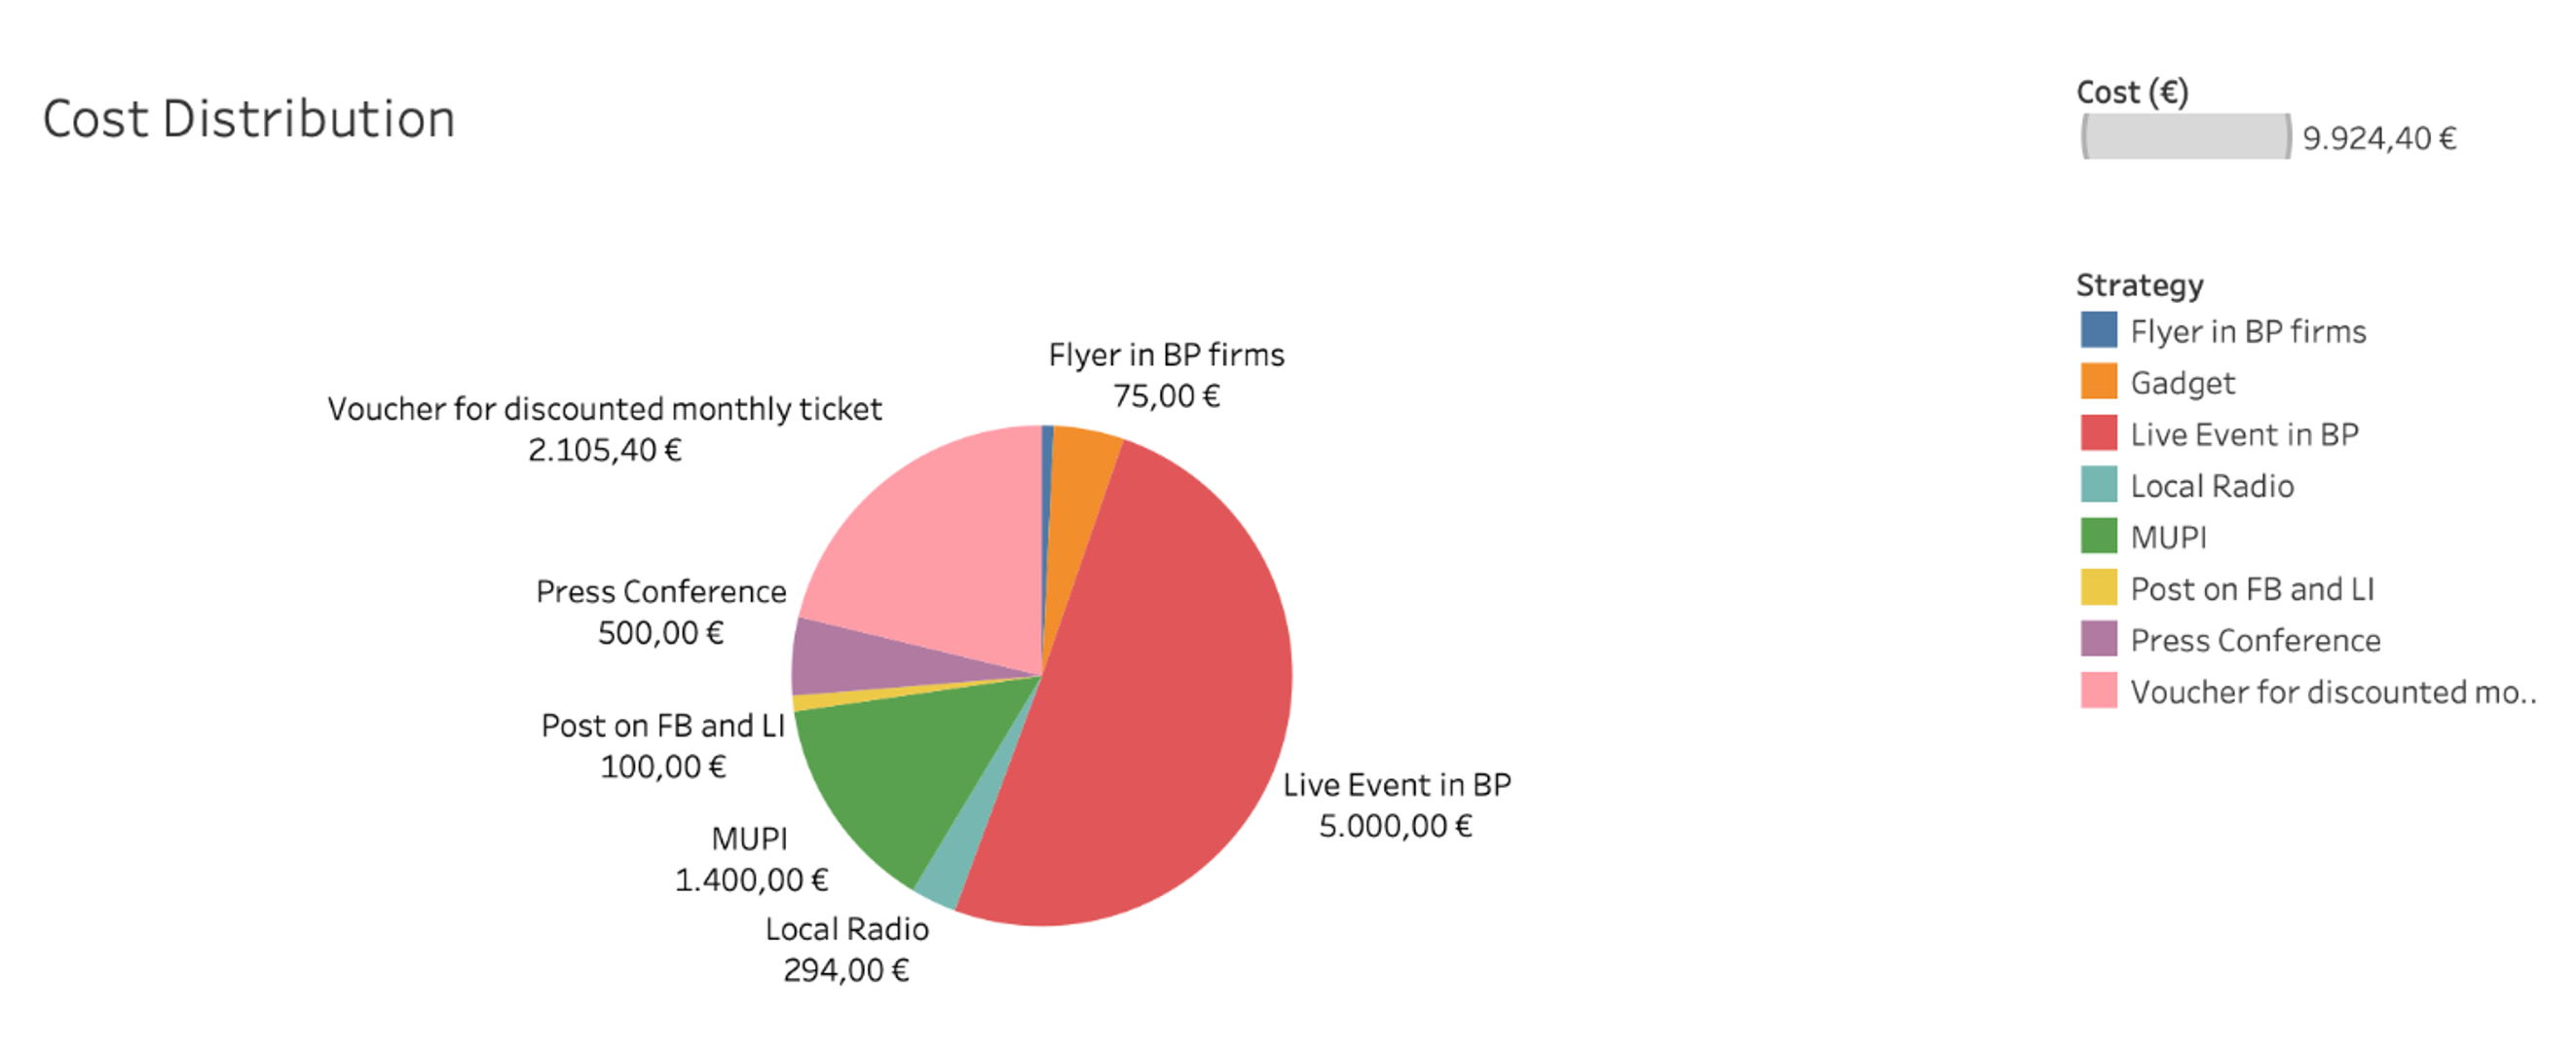
\includegraphics[width=0.8\textwidth]{Images/merketing/cost_distribution.png}
    \caption{Costs Distribution}
    \label{fig:costdistribution}
\end{figure}

The launch of the new service is scheduled on the 10th of October, as previously mentioned. The marketing campaign starts six weeks before the launch of the service. The first two initiatives to be implemented are the publication of posts on social media, like Facebook and LinkedIn, and the wrapping on buses serving the line from Voghera to Stradella, line that will be modified for the Business Park service. The former is intended to reach the so called “white collars” of the Business Park, while the latter is targeting the pedestrians and drivers in the towns near the Business Park, that may come into contact with the wrapped buses. Both strategies start at the beginning of September to enhance the level of exposition and reach the highest number of potential customers. The wrapping process for 20 buses requires a week, thus the buses will be ready on 09/09. The posts on social media will be weekly monitored till the end of the marketing campaign, collecting the number of reactions and likes to measure the impact of the action.

The most institutional marketing measure for our stakeholders consists in a press conference on the 3/10; its preparation is estimated lasting 14 days, to find a location, invite journalists and set up the speech. During the press conference, gadgets will be distributed. They are made since the 11th September, to have 21 days of preparation and have them ready for the press event. The efficacy of the press will be monitored with the number of articles on the newspaper, weighted by the average number of copies sold.

The Business Park Live Event is organized two days before the New Service Launch, on a Saturday evening, to guarantee the highest participation of employees and workers. The estimated duration of its preparation is 35 days starting from the 03/09/22, to obtain the permission, find the catering and organize family entertainment during the evening. The effectiveness of this event is measured with two metrics: for the month of October with the ratio of used over emitted voucher, distributed during the event. For the month of November, on the other hand, the suggested KPI is the renovated monthly ticket over the original emitted voucher to get an indication of the initial customer loyalty for the new service.

Since the vouchers are distributed during the Live Event, and the expected duration for the administrative works is 21 days, their preparation starts on the 17/09/22.

Another item connected to the Live Event is the flyers. These will be hanged on boards inside the companies in the Business Park one week before the Live Event, and they require a week for their preparation.

The spots on Radio Voghera are scheduled for the last two weeks before the start of the new service in order to try to engage those who “were left behind” with the previous measures. Moreover, radiophonic spots can be effective to target a particular market segment: car users. 

Three spots per day are planned. The effectiveness of this action is measured by the average share of audience for each day on Radio Voghera during the spots airing.
\begin{figure}
    \centering
    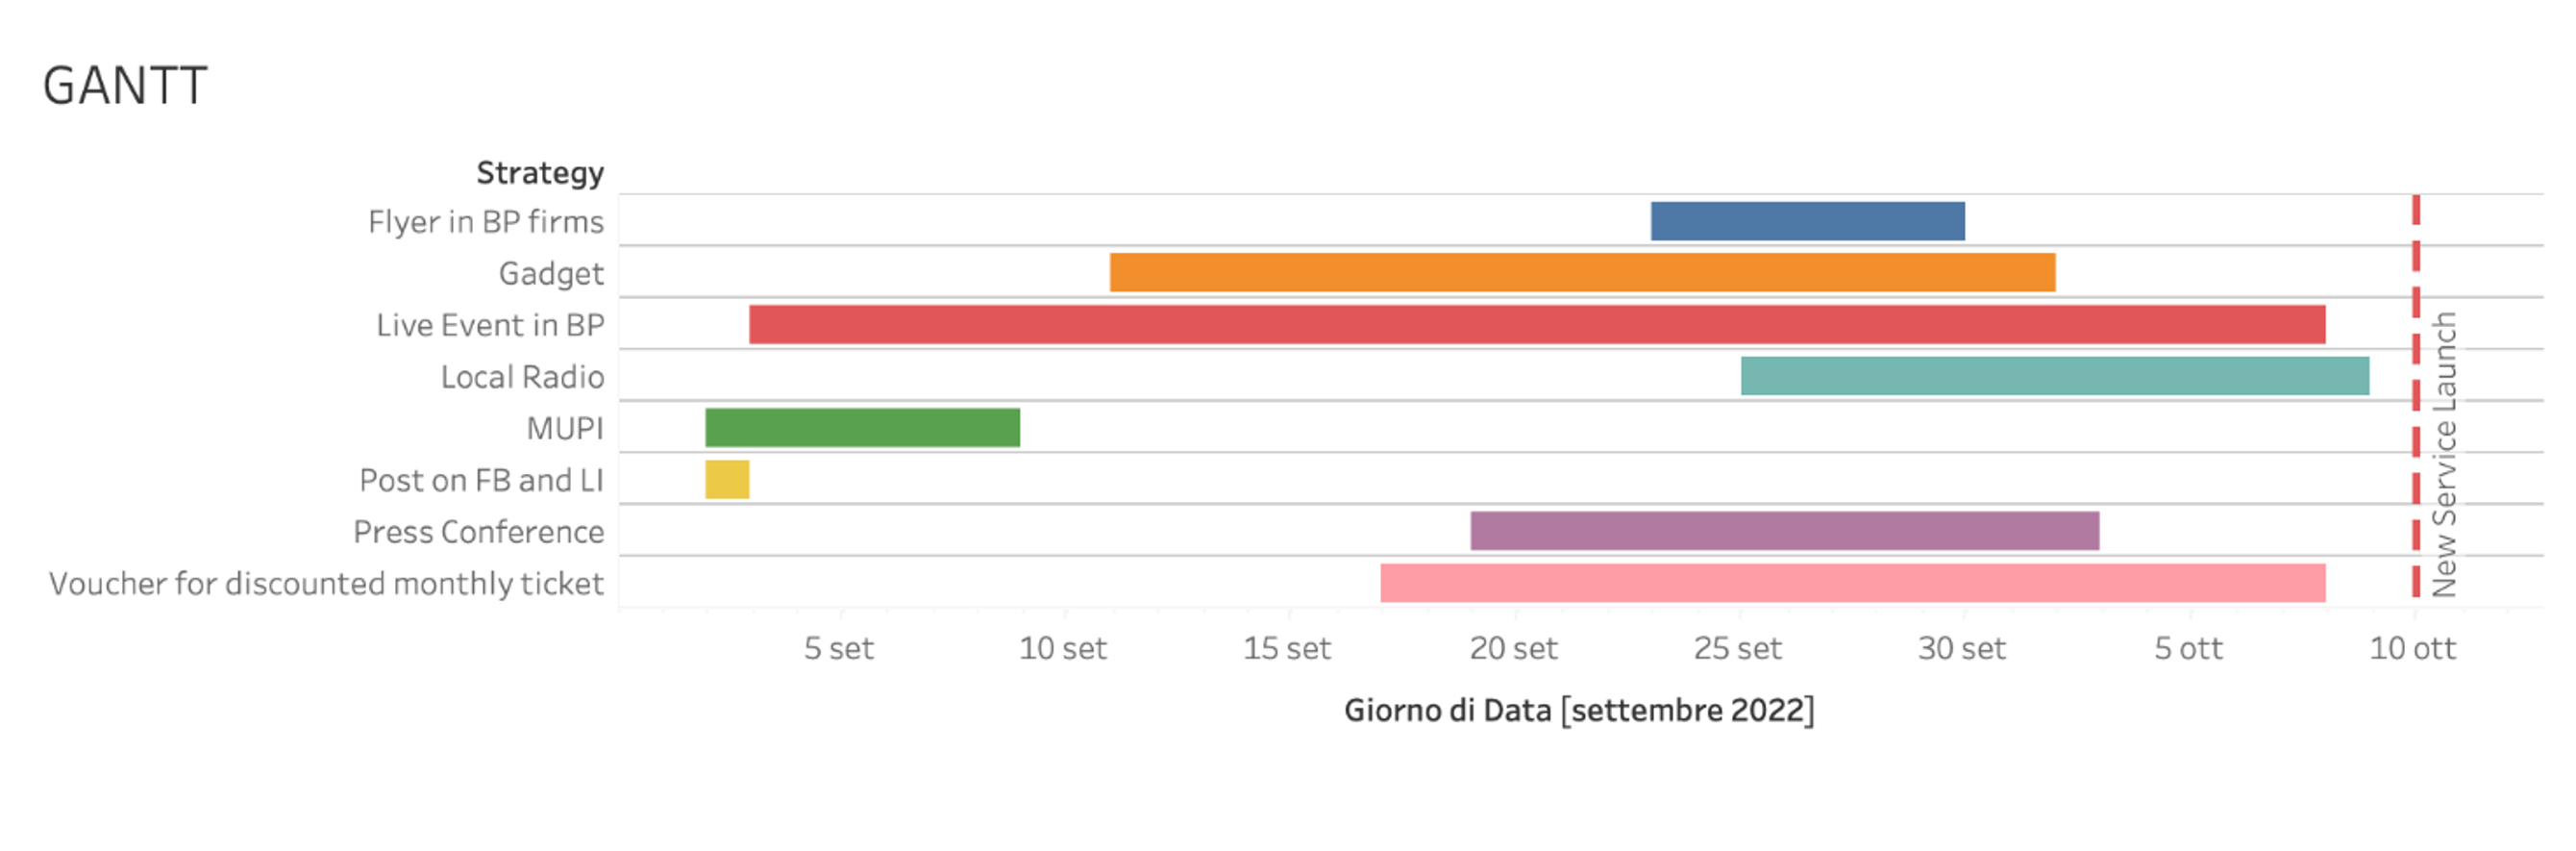
\includegraphics[width=0.8\textwidth]{Images/merketing/gantt.png}
    \caption{GANTT Chart }
    \label{fig:gantt}
\end{figure}

For all the measures for which is difficult to find a synthetic KPI, like gadget and bus wrapping, surveys and interviews are suggested at the end of the Live Event and for the first weeks of the new bus service. These polls should enable the company to understand how customers got to know the new service and understand which measures were the most appreciated and effective ones, both from an advertising and economic perspective.

